\section{设计方案}

\subsection{总体设计思路}

\begin{figure}[H]
  \centering
  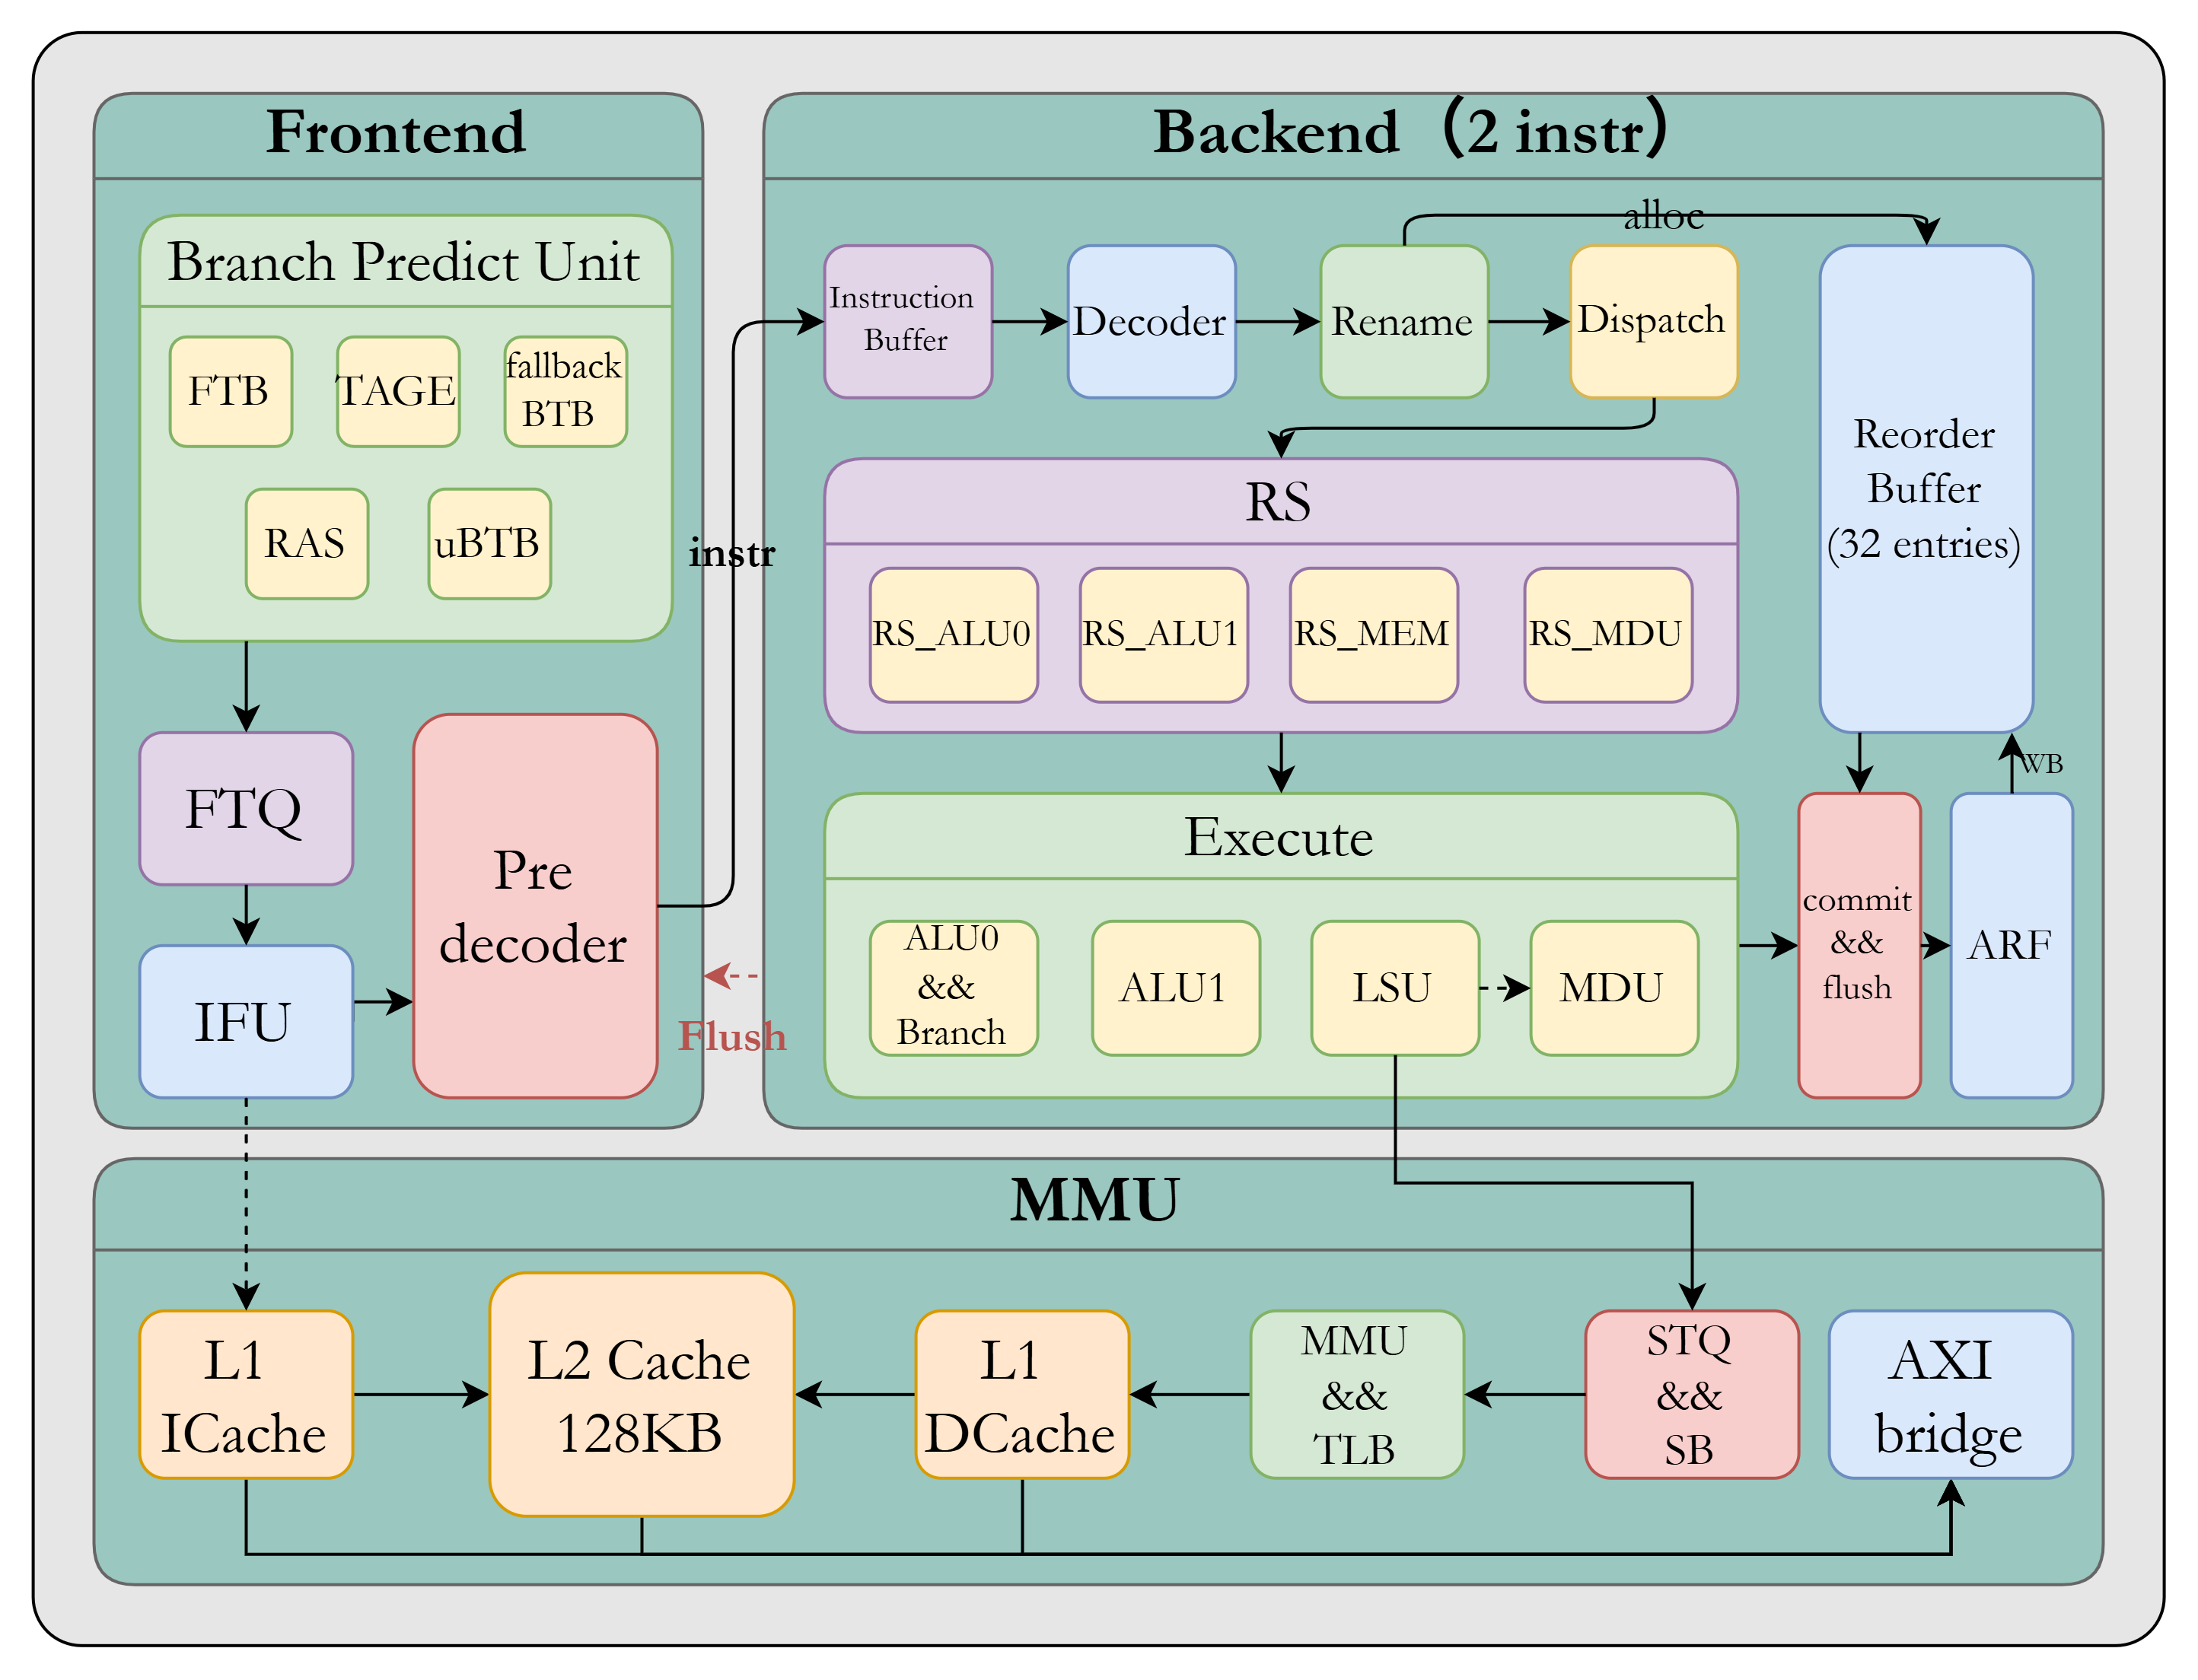
\includegraphics[width=0.98\textwidth]{figure/mycpu_arch.png}
  \caption{CPU 设计架构图}
  \label{fig:cpuarch}
\end{figure}

前端可划分为分支预测与取指两大部分：分支预测包含 uBTB、fallback BTB、FTB、TAGE、RAS 等组件；取指路径为 FTQ $\rightarrow$ IFU（含预译码）$\rightarrow$ ICache $\rightarrow$ 指令缓冲（IB），每拍最多向 IB 填入 4 条指令。

后端从流水级上看分为译码、重命名、分发、保留站发射、执行与提交；从功能上看包含译码器（decoder$\times$2）、指令缓冲（IB）、寄存器别名表（RAT）、架构寄存器堆（ARF）、重排序缓存（ROB）、分发单元（dispatch）、三类保留站（RS\_ALU$\times$2、RS\_MEM、RS\_MDU）以及执行单元 ALU$\times$2、LSU、MDU，并由提交级与ctrl（控制冲刷）统一处理误预测、异常与特权副作用。

指令执行过程大致如下：
\begin{enumerate}
  \item \textbf{译码}：每拍从 IB 最多取两条指令，生成 FU 类型、操作码、立即数、特权向量与例外信息；
  \item \textbf{重命名}：查询/更新 RAT，以 ROB 编号作为源/目的寄存器的重命名标签（无 PRF 与 freelist），并成对分配 ROB 项（双发所以成对分配）；
  \item \textbf{分发}：从 ROB 补齐就绪操作数，将指令路由至对应保留站；
  \item \textbf{发射与执行}：ALU 保留站乱序发射到双 ALU（含分支判定）；访存与乘除杂项经各自 FIFO 保留站进入 LSU/MDU；结果写回 ROB；
  \item \textbf{提交}：检查 ROB 队头至多两条指令是否可退休，完成写 ARF、CSR/TLB 维护、Store Buffer 入队、分支训练以及异常/误预测冲刷。
\end{enumerate}

各容量概览见表~\ref{tab:capacity}。

\begin{table}[H]
\centering
\caption{容量概览}
\label{tab:capacity}
\small
\begin{tabular}{>{\raggedright\arraybackslash}p{3.2cm}>{\raggedright\arraybackslash}p{11.8cm}}
\toprule
结构 & 规格 \\
\midrule
取指 / 后端宽度 & 4 宽基本块取指 / 2 宽译码与提交 \\
ROB & 32 项（分奇偶两部分，一部分 16 项，共 16 对） \\
IB / FTQ & 16 项 / 16 项 \\
RS & ALU$\times$2 各 4 项；MEM 4 项；MDU 2 项 \\
STQ / Store Buffer & 16 / 8 \\
Icache / Dcache & 各 16\,KB，4 路$\times$128 组$\times$32\,B，VIPT \\
L2 & 128\,KB，2 路$\times$2048 组$\times$32\,B \\
TLB & 主 TLB 32 项双查口；I/D L1 微 TLB 各 8 项 \\
BPU & uBTB 16；fallback BTB 64；FTB $4\times2048$；TAGE 8K$+$4$\times$1K；RAS 32 双栈 \\
\bottomrule
\end{tabular}
\end{table}

\subsubsection{指令实现}

按照指令类型，意味核实现了如下指令（见表~\ref{tab:inst}）。
其中 \texttt{ibar}/\texttt{dbar} 译码为特权屏障标记，提交时等待 Store Buffer 排空后发起重取冲刷；
\texttt{preld} 被识别为已知指令并以空操作退休（不做硬件预取），从而不触发 INE。

\begin{table}[H]
\centering
\caption{指令实现}
\label{tab:inst}
\small
\begin{tabular}{>{\raggedright\arraybackslash}p{3.2cm}>{\raggedright\arraybackslash}p{11.5cm}}
\toprule
指令类型 & 指令名称 \\
\midrule
算术运算类指令 &
\texttt{add.w}, \texttt{sub.w}, \texttt{addi.w}, \texttt{slt}, \texttt{sltu}, \texttt{slti}, \texttt{sltui},
\texttt{lu12i.w}, \texttt{pcaddu12i}, \texttt{and}, \texttt{or}, \texttt{nor}, \texttt{xor},
\texttt{andi}, \texttt{ori}, \texttt{xori}, \texttt{mul.w}, \texttt{mulh.w}, \texttt{mulh.wu},
\texttt{div.w}, \texttt{div.wu}, \texttt{mod.w}, \texttt{mod.wu} \\
移位运算类指令 &
\texttt{sll.w}, \texttt{srl.w}, \texttt{sra.w}, \texttt{slli.w}, \texttt{srli.w}, \texttt{srai.w} \\
分支跳转指令 &
\texttt{beq}, \texttt{bne}, \texttt{blt}, \texttt{bltu}, \texttt{bge}, \texttt{bgeu}, \texttt{b}, \texttt{bl}, \texttt{jirl} \\
普通访存指令 &
\texttt{ld.b}, \texttt{ld.bu}, \texttt{ld.h}, \texttt{ld.hu}, \texttt{ld.w}, \texttt{st.b}, \texttt{st.h}, \texttt{st.w} \\
原子访存指令 & \texttt{ll.w}, \texttt{sc.w} \\
屏障与预取 & \texttt{ibar}, \texttt{dbar}, \texttt{preld} \\
特权指令 &
\texttt{csrrd}, \texttt{csrwr}, \texttt{csrxchg}, \texttt{tlbsrch}, \texttt{tlbrd}, \texttt{tlbwr},
\texttt{tlbfill}, \texttt{invtlb}, \texttt{cacop}, \texttt{ertn}, \texttt{idle} \\
系统异常指令 & \texttt{syscall}, \texttt{break} \\
计时器相关指令 & \texttt{rdcntid}, \texttt{rdcntvl.w}, \texttt{rdcntvh.w} \\
读取配置指令 & \texttt{cpucfg} \\
\bottomrule
\end{tabular}
\end{table}

\subsubsection{CSR 实现}

意味核实现了以上全部指令所需的 CSR，具体如表~\ref{tab:csr}。
未实现编号的 CSR 读返回 0、写忽略。部分低风险 CSR（如 TICLR、SAVE0--3、TID）采用 L0 写路径，提交后无需全局重取。

\begin{table}[H]
\centering
\caption{CSR 实现}
\label{tab:csr}
\small
\begin{tabular}{cll|cll}
\toprule
地址 & 含义 & 名称 & 地址 & 含义 & 名称 \\
\midrule
0x0 & 当前模式信息 & CRMD & 0x30--33 & 数据保存 & SAVE0--3 \\
0x1 & 例外前模式信息 & PRMD & 0x40 & 定时器编号 & TID \\
0x2 & 扩展组件使能 & EUEN & 0x41 & 定时器配置 & TCFG \\
0x4 & 例外配置 & ECFG & 0x42 & 定时器值 & TVAL \\
0x5 & 例外状态 & ESTAT & 0x44 & 定时中断清除 & TICLR \\
0x6 & 例外返回地址 & ERA & 0x60 & LLBit 控制 & LLBCTL \\
0x7 & 出错虚地址 & BADV & 0x88 & TLB 重填入口 & TLBRENTRY \\
0xC & 例外入口地址 & EENTRY & 0x180--181 & 直接映射窗口 & DMW0--1 \\
0x10 & TLB 索引 & TLBIDX & 0x18 & ASID & ASID \\
0x11 & TLB 表项高位 & TLBEHI & 0x19 & 低半目录基址 & PGDL \\
0x12 & TLB 表项低位 0 & TLBELO0 & 0x1A & 高半目录基址 & PGDH \\
0x13 & TLB 表项低位 1 & TLBELO1 & 0x1B & 全局目录基址 & PGD \\
0x20 & 处理器编号 & CPUID & & & \\
\bottomrule
\end{tabular}
\end{table}

\subsubsection{例外与中断}

本处理器支持 LoongArch-32R 手册要求的主要例外与中断，如表~\ref{tab:excp}。
例外在流水中附着于指令，于提交级按优先级编码后写入 CSR 并冲刷前端。而中断则附着在即将提交的指令上处理。\texttt{idle} 提交后冻结取指，直至中断到来。

\begin{table}[H]
\centering
\caption{例外与中断}
\label{tab:excp}
\begin{tabular}{cccc}
\toprule
Ecode & Esubcode & 例外代号 & 例外类型 \\
\midrule
0x0 & 0 & INT & 中断 \\
0x1 & 0 & PIL & load 操作页无效例外 \\
0x2 & 0 & PIS & store 操作页无效例外 \\
0x3 & 0 & PIF & 取指操作页无效例外 \\
0x4 & 0 & PME & 页修改例外 \\
0x7 & 0 & PPI & 页特权等级不合规例外 \\
0x8 & 0 & ADEF & 取指地址错例外 \\
0x9 & 0 & ALE & 地址非对齐例外 \\
0xB & 0 & SYS & 系统调用例外 \\
0xC & 0 & BRK & 断点例外 \\
0xD & 0 & INE & 指令不存在例外 \\
0x3F & 0 & TLBR & TLB 重填例外 \\
\bottomrule
\end{tabular}
\end{table}

\subsubsection{地址翻译模式}

意味核支持直接地址翻译、直接映射地址翻译与页表映射地址翻译三种模式。

当 \texttt{CSR.CRMD} 中 DA$=1$ 且 PG$=0$ 时为直接地址翻译，物理地址等于虚拟地址。
当 DA$=0$ 且 PG$=1$ 时进入映射模式：若虚地址命中有效 DMW 窗口，则按窗口配置拼接物理地址高位；否则查询 TLB。
命中有效 TLB 表项则完成翻译，否则触发 TLB 重填例外。
取指与访存通路各自经过 MMU 门面，并配备 L1 微 TLB 加速常用 4\,KB 页翻译。
